\documentclass[12pt]{article}
\usepackage{amsfonts, epsfig}
\usepackage{booktabs} % for better table formatting
\usepackage[authoryear]{natbib}
\usepackage{array}
\usepackage{multirow}
\usepackage{graphicx}
\usepackage{fancyhdr}
\pagestyle{fancy}
\lfoot{\texttt{ematm0067.github.io} / \texttt{ematm0044.github.io}}
\lhead{Introduction to AI - 02.3\_regression - Conor}
\rhead{\thepage}
\cfoot{}

\usepackage{tikz}
\usetikzlibrary{positioning}

\usepackage{ifthen}
\newboolean{nopics}
\setboolean{nopics}{true}


\begin{document}

\section*{Linear regression.} 

Recently when doing some research, the details of which are not
relevant here, I measured the relationship between two variables, here
I will just call them $x$ and $y$. The data look like:
\begin{center}
\begin{tabular}{@{}ccccccccc@{}}
\toprule
x & 8 & 9 & 10 & 11 & 12 & 13 & 14 & 15 \\ \midrule
y & 54 & 69 & 75 & 78 & 85 & 102 & 103 & 103 \\ \bottomrule
\end{tabular}
\end{center}
When I plotted these data I was surprised, I had expect it to look
roughly like
\begin{equation}
  y\propto 2^x
\end{equation}
but, as is clear from the scatterplot
\begin{center}
  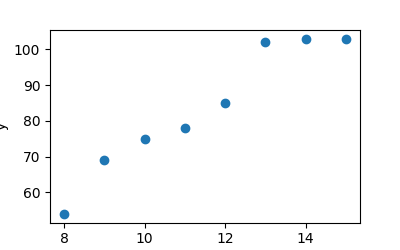
\includegraphics[]{02.3_points.png}
  \end{center}
that it looks a lot more like
\begin{equation}
  y=mx+c
\end{equation}
for some $m$ and $c$. In linear regression we find the values $m$ and
$c$ to give the best line to describe data. This, clearly, raises the
question as to what we mean by best, it also begs the question as to
whether we will know the linear model is a good description or not. We
will answer the first question straight away, the second question is
trickier and we won't consider that here: our intention here is to
find the best line for describing the data under the assumption that
that is a useful thing to do. In practice, data are often described by
a linear model and, if they are, linear models are very easy to use,
so it is often useful to try a linear model first!

The approach we take to deciding what we mean by the `best' line is to
think of the line as a prediction, we think of it as model for the
data, so for each $x$ we have a prediction:
\begin{equation}
  \hat{y}=mx+c
\end{equation}
and this prediction has an error $|\hat{y}-y|$.
\begin{center}
  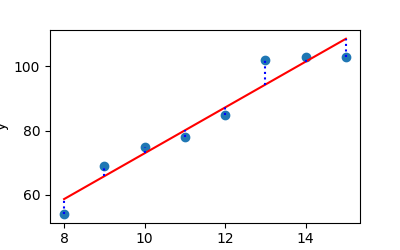
\includegraphics[]{02.3_points_line.png}
  \end{center}
It is typical for models to not make completely accurate predictions,
we imagine that there is some process that is largely responsible for
generating $y$ from $x$ but there is noise: we know that we should
expect the position for an object moving at a constant speed $v$ to be
$vt$, but we also accept that in practice wind or whatever will make
that approximate and our measurement of the position will not be
completely accurate. Nonetheless, we clearly want to minimize the
noise.

However, this does not fully specify what we mean by the error, one
idea would be to sum the individual errors:
\begin{equation}
  \mathcal{E}_1=\frac{1}{n}\sum_i |\hat{y}_i-y|
\end{equation}
where, in the obvious way $\hat{y}_i=mx_i+c$. In fact this would be
very inconvenient because the absolute value can be an awkward object; it has long been common to use the \textsl{root mean square error} instead:
\begin{equation}
  \mathcal{E}_2=\sqrt{\frac{1}{n}\sum_i (\hat{y}_i-y)^2}
\end{equation}
We will see shortly that using the square makes the mathematics of
finding $m$ and $c$ easier, but picking $\mathcal{E}_2$ over
$\mathcal{E}_1$, or indeed over any other error function including
\begin{equation}
  \mathcal{E}_p=\sqrt[p]{\frac{1}{n}\sum_i (\hat{y}_i-y)^2}
\end{equation}
In fact, along with the practical impetus to using $\mathcal{E}_2$,
there is a principled argument based on models of the noise and the
nature of prediction which describes reasonably generic circumstances
where it is the best choice. We will not go into that here.

So, we have decided our task is to pick the $m$ and $c$ that minimize
$\mathcal{E}_2$. In fact, we will consider $\mathcal{E}_2^2$, the
\textsl{mean square error} instead: since the square root is a
monotonically increasing function the values of $m$ and $c$ that
minimize $\mathcal{E}_2^2$ will also minimize
$\mathcal{E}_2$. Substituting in for $\hat{y}_i$ we want to minimize
\begin{equation}
\mathcal{E}_2^2=\frac{1}{n}\sum_i(mx_i+c-y_i)^2
\end{equation}
To minimize we use calculus, a necessary condition for a minimum is that the partial derivatives vanish:
\begin{equation}
\frac{\partial \mathcal{E}_2^2}{\partial m}=\frac{\partial \mathcal{E}_2^2}{\partial c}=0
\end{equation}
Obviously this does not rule out the possibility of a saddlepoint or
maximum, but in this example we are fortunate, looking at the form of
$\mathcal{E}_2^2$ is should be clear that any stationary point is a
minimum, this is easy enough to prove with second order derivatives,
but we won't go into that here.

The derivatives are easy enough using the chain rule, to remind you,
if $f(x)=d(u(x))$ then the rate of change of $f$ with $x$ is the
multiple of how $f$ changes with $u$ and how $u$ changes with $x$:
\begin{equation}
\frac{df}{dx}=\frac{df}{du}\frac{du}{dx}
\end{equation}
The chain rule is easy to remember because it sort of makes sense but
it is also incredibly powerful, allowing any calculation you can
perform to be differentiated. As an aside this is the essence of
\textt{autograd}, the automatic differentiation routines that make
modern machine learning possible. 

In the case here let $u_i=mx_i+c-y_i$ so
\begin{equation}
\mathcal{E}_2^2=\frac{1}{n}\sum_iu_i^2
\end{equation}
and
\begin{equation}
\frac{\partial \mathcal{E}_2^2}{\partial c}=\sum_i\frac{\partial u_i^2}{\partial c}=\sum_i\frac{d u_i^2}{du_i}\frac{\partial u_i}{\partial c}=2\sum_i u_i
\end{equation}
since the derivative of $u_i$ with respect to $c$ is just one. Hence,
one of the two conditions is
\begin{equation}
0=\sum_i u_i = m\frac{1}{n}\sum_i x_i + c\frac{1}{n}\sum_i 1-\frac{1}{n}\sum_i y_i
\end{equation}
and using a bar for the sample mean of a quantity:
\begin{equation}
\bar{z}=\frac{1}{n}\sum_i z_i
\end{equation}
we get
\begin{equation}
m\bar{x}+c=\bar{y}
\end{equation}
 


\section*{Summary}

\end{document}

